\documentclass[aspectratio=169,10pt]{beamer}

\usepackage[T1]{fontenc}
\usepackage[utf8]{inputenc}
\usepackage[brazilian]{babel}
\usepackage{helvet}
\usepackage{graphicx}
\usepackage{booktabs}
\usepackage{tikz}
\usepackage{pgfplots}
\usepackage{amsmath}
\usepackage{microtype}

\pgfplotsset{compat=1.18}
\renewcommand{\familydefault}{\sfdefault}

\definecolor{ufpidark}{HTML}{006633}
\definecolor{ufpilight}{HTML}{6A963F}
\definecolor{ink}{HTML}{20252A}
\definecolor{muted}{HTML}{657078}
\definecolor{soft}{HTML}{E8ECE9}
\definecolor{pale}{HTML}{F5F7F5}

\setbeamercolor{normal text}{fg=ink,bg=white}
\setbeamercolor{structure}{fg=ufpidark}
\setbeamercolor{frametitle}{fg=ink,bg=white}
\setbeamercolor{alerted text}{fg=ufpidark}
\setbeamercolor{footline}{fg=muted,bg=white}
\setbeamerfont{frametitle}{size=\fontsize{22.5}{26}\selectfont,series=\bfseries}
\setbeamerfont{normal text}{size=\fontsize{16}{20}\selectfont}
\setbeamerfont{footline}{size=\scriptsize}
\setbeamertemplate{navigation symbols}{}
\setbeamertemplate{itemize item}{\color{ufpidark}\rule[0.4ex]{0.7ex}{0.7ex}}
\setbeamertemplate{itemize subitem}{\color{ufpilight}\rule[0.4ex]{0.55ex}{0.55ex}}
\setbeamertemplate{frametitle}{%
  \vspace{0.32cm}\insertframetitle\par
  \vspace{0.12cm}{\color{ufpilight}\rule{1.15cm}{1.8pt}}
}
\setbeamertemplate{footline}{%
  \leavevmode
  \hbox{%
    \begin{beamercolorbox}[wd=.86\paperwidth,ht=2.7ex,dp=1.2ex,leftskip=.55cm]{footline}%
      TACO + YOLO26n \hspace{0.7em} \textcolor{soft}{|} \hspace{0.7em} UFPI -- Campus Picos
    \end{beamercolorbox}%
    \begin{beamercolorbox}[wd=.14\paperwidth,ht=2.7ex,dp=1.2ex,rightskip=.55cm plus1fil]{footline}%
      \hfill\insertframenumber/\inserttotalframenumber
    \end{beamercolorbox}%
  }
}

\newcommand{\source}[1]{%
  \par\vspace{0.15cm}{\color{muted}\fontsize{8.5}{10}\selectfont Fonte: #1}
}
\newcommand{\bigmetric}[2]{%
  {\color{ufpidark}\fontsize{24}{27}\selectfont\bfseries #1}\par
  \vspace{0.03cm}{\color{muted}\fontsize{10.5}{13}\selectfont #2}
}

\title{O custo da granularidade semântica\\na detecção de resíduos}
\subtitle{Estudo controlado com TACO e YOLO26n}
\author{Jean Carlos Rodrigues Sousa, Karielly de Carvalho, Marcos A. G. B. Brito}
\institute{Universidade Federal do Piauí -- Campus Senador Helvídio Nunes de Barros}

\begin{document}

% 1
\begin{frame}[plain]
  \vfill
  \begin{columns}[c,onlytextwidth]
    \begin{column}{0.77\textwidth}
      {\color{ufpidark}\fontsize{10.5}{12}\selectfont UNIVERSIDADE FEDERAL DO PIAUÍ}\par
      \vspace{0.34cm}
      {\fontsize{24}{28}\selectfont\bfseries O custo da granularidade\\semântica na detecção de resíduos}\par
      \vspace{0.18cm}
      {\color{muted}\fontsize{15}{18}\selectfont Estudo controlado com TACO e YOLO26n}\par
      \vspace{0.48cm}
      {\fontsize{11.5}{14}\selectfont Jean Carlos Rodrigues Sousa\quad Karielly de Carvalho\\Marcos A. G. B. Brito}\par
      \vspace{0.10cm}
      {\color{muted}\fontsize{9.5}{11}\selectfont UFPI -- CSHNB, Picos--PI}
    \end{column}
    \begin{column}{0.20\textwidth}
      \hfill
\includegraphics[width=0.78\linewidth]{assets/ufpi_brasao.png}
    \end{column}
  \end{columns}
  \vfill
  {\color{ufpilight}\rule{\textwidth}{2.2pt}}
\end{frame}

% 2
\begin{frame}{Pergunta central}
  \vspace{0.3cm}
  {\fontsize{24}{31}\selectfont\bfseries
  Como a granularidade das classes afeta a detecção em um conjunto pequeno e de cauda longa?}

  \vspace{0.65cm}
  \begin{columns}[T,onlytextwidth]
    \begin{column}{0.47\textwidth}
      {\color{ufpidark}\bfseries Localização}\par
      \vspace{0.12cm}
      O modelo precisa encontrar o resíduo e delimitar sua posição.
    \end{column}
    \begin{column}{0.47\textwidth}
      {\color{ufpidark}\bfseries Semântica}\par
      \vspace{0.12cm}
      A mesma caixa pode ser penalizada quando recebe um rótulo incorreto.
    \end{column}
  \end{columns}

  \vspace{0.65cm}
  {\color{muted}\fontsize{13}{16}\selectfont O experimento mantém imagens, caixas, partição e treinamento constantes. Somente a taxonomia muda.}
\end{frame}

% 3
\begin{frame}{TACO e o problema de cauda longa}
  \vspace{-0.08cm}
  \begin{columns}[T,onlytextwidth]
    \begin{column}{0.30\textwidth}
      \bigmetric{1.500}{imagens em ambientes reais}
    \end{column}
    \begin{column}{0.30\textwidth}
      \bigmetric{4.784}{objetos anotados}
    \end{column}
    \begin{column}{0.30\textwidth}
      \bigmetric{60}{classes Fine oficiais}
    \end{column}
  \end{columns}
  \vspace{0.15cm}
  \begin{columns}[c,onlytextwidth]
    \begin{column}{0.64\textwidth}
      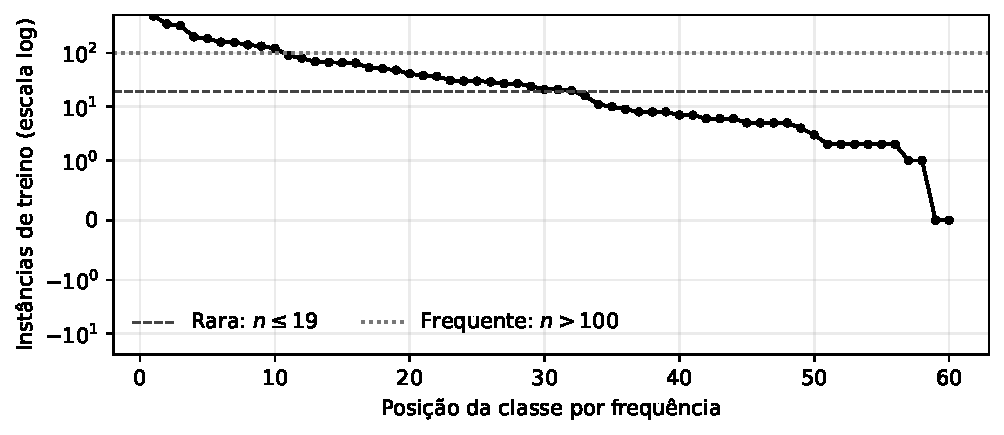
\includegraphics[width=\linewidth]{../paper/figures/class_rank_distribution.pdf}
    \end{column}
    \begin{column}{0.32\textwidth}
      {\color{ufpidark}\fontsize{15}{18}\selectfont\bfseries Cauda longa}\par
      \vspace{0.12cm}
      {\fontsize{12.5}{15}\selectfont Poucas classes concentram muitos exemplos, enquanto várias categorias possuem amostras escassas.}
    \end{column}
  \end{columns}
  \vspace{-0.05cm}
  \source{Proença e Simões (2020); distribuição calculada na partição de treino.}
\end{frame}

% 4
\begin{frame}{Como o TACO representa cada objeto}
  \vspace{0.01cm}
  \begin{columns}[T,onlytextwidth]
    \begin{column}{0.205\textwidth}
      \centering{\color{ufpidark}\bfseries Imagem original}\par\vspace{0.10cm}
      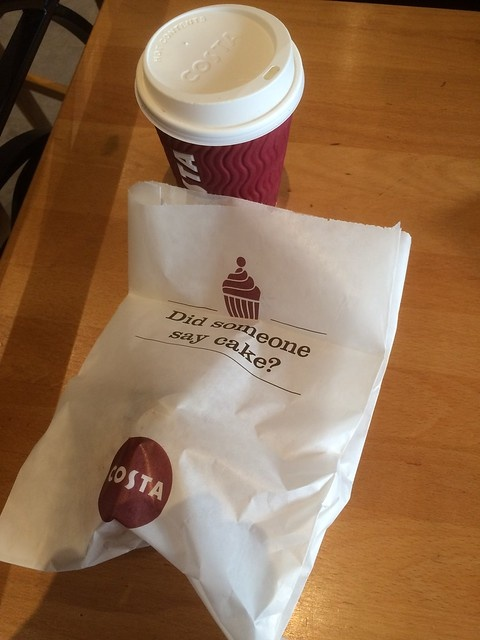
\includegraphics[height=3.58cm,width=\linewidth,keepaspectratio]{assets/taco_original_example.png}
    \end{column}
    \begin{column}{0.205\textwidth}
      \centering{\color{ufpidark}\bfseries Segmentação Fine}\par\vspace{0.10cm}
      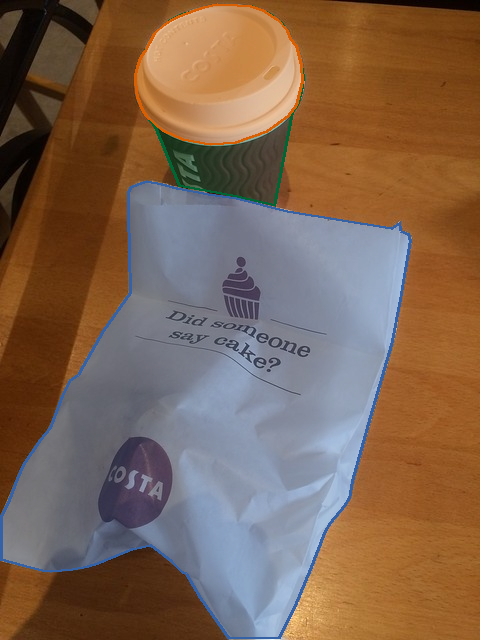
\includegraphics[height=3.58cm,width=\linewidth,keepaspectratio]{assets/taco_segmentation_example.png}
    \end{column}
    \begin{column}{0.205\textwidth}
      \centering{\color{ufpidark}\bfseries Caixas COCO}\par\vspace{0.10cm}
      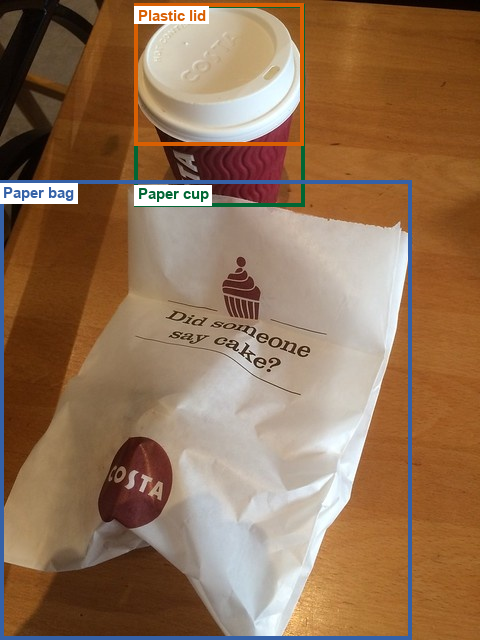
\includegraphics[height=3.58cm,width=\linewidth,keepaspectratio]{assets/taco_bbox_example.png}
    \end{column}
    \begin{column}{0.31\textwidth}
      {\fontsize{14}{17}\selectfont\bfseries O JSON fornece}\par
      \vspace{0.08cm}
      {\fontsize{11}{14}\selectfont Máscara poligonal\\Caixa delimitadora\\Categoria Fine}\par
      \vspace{0.14cm}
      {\color{ufpidark}\fontsize{13}{16}\selectfont\bfseries Remapeamento}\par
      \vspace{0.06cm}
      {\fontsize{10.5}{13}\selectfont
      Paper cup $\rightarrow$ Paper/Cardboard $\rightarrow$ Litter\\[0.06cm]
      Plastic lid $\rightarrow$ Plastic $\rightarrow$ Litter}
      \vspace{0.18cm}

      {\color{muted}\fontsize{9.5}{12}\selectfont 3 objetos e 3 classes Fine. O YOLO utiliza as caixas; as máscaras documentam a anotação original.}
    \end{column}
  \end{columns}
\end{frame}

% 5
\begin{frame}{Desenho experimental controlado}
  \vspace{-0.10cm}
  \begin{columns}[c,onlytextwidth]
    \begin{column}{0.72\textwidth}
      \centering
      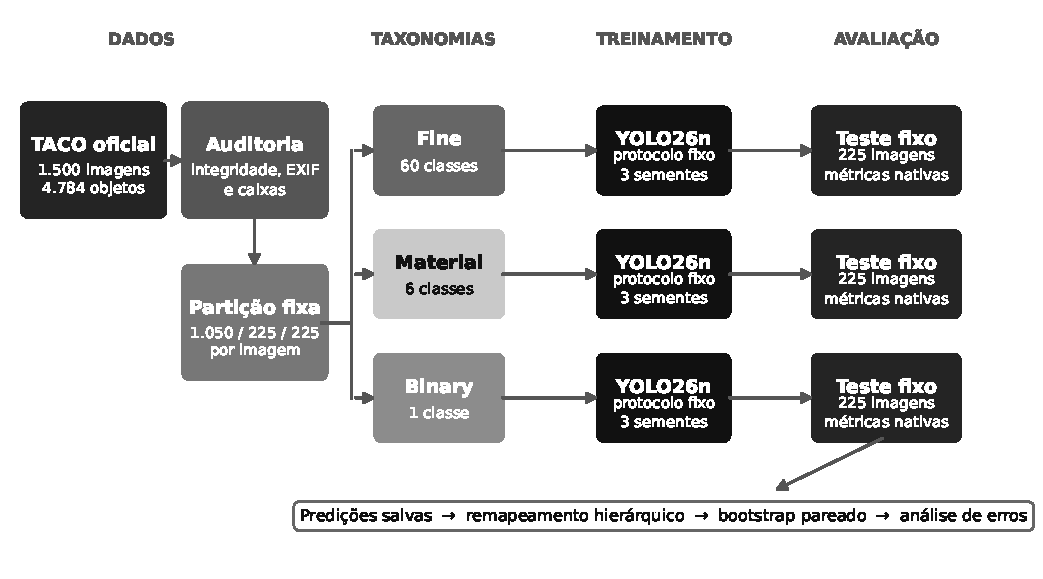
\includegraphics[height=5.05cm,width=\linewidth,keepaspectratio]{../paper/figures/methodology_pipeline.pdf}
    \end{column}
    \begin{column}{0.25\textwidth}
      {\color{ufpidark}\bfseries Partição fixa}\par
      \vspace{0.06cm}{\fontsize{11}{13}\selectfont 1.050 treino\\225 validação\\225 teste}\par
      \vspace{0.28cm}
      {\color{ufpidark}\bfseries YOLO26n}\par
      \vspace{0.06cm}{\fontsize{11}{13}\selectfont Entrada 640\\Lote 24\\Até 60 épocas}\par
      \vspace{0.28cm}
      {\color{ufpidark}\bfseries Sementes}\par
      \vspace{0.06cm}{\fontsize{11}{13}\selectfont 42, 123 e 2026}
    \end{column}
  \end{columns}
\end{frame}

% 6
\begin{frame}{Três níveis de detalhe semântico}
  \vspace{0.35cm}
  \begin{columns}[T,onlytextwidth]
    \begin{column}{0.30\textwidth}
      {\color{ufpidark}\fontsize{29}{32}\selectfont\bfseries 60}\par
      {\fontsize{18}{22}\selectfont\bfseries Fine}\par
      \vspace{0.22cm}
      Categorias oficiais, como lata de alumínio, garrafa de vidro e tampa plástica.
    \end{column}
    \begin{column}{0.03\textwidth}
      \centering{\color{soft}\rule{1pt}{4.2cm}}
    \end{column}
    \begin{column}{0.31\textwidth}
      {\color{ufpidark}\fontsize{29}{32}\selectfont\bfseries 6}\par
      {\fontsize{18}{22}\selectfont\bfseries Material}\par
      \vspace{0.22cm}
      Plastic, Metal, Glass, Paper/Cardboard, Organic e Other.
    \end{column}
    \begin{column}{0.03\textwidth}
      \centering{\color{soft}\rule{1pt}{4.2cm}}
    \end{column}
    \begin{column}{0.30\textwidth}
      {\color{ufpidark}\fontsize{29}{32}\selectfont\bfseries 1}\par
      {\fontsize{18}{22}\selectfont\bfseries Binary}\par
      \vspace{0.22cm}
      Todo objeto recebe o rótulo \textit{Litter}. A tarefa preserva apenas resíduo versus fundo.
    \end{column}
  \end{columns}
  \vfill
  {\color{muted}\fontsize{12.5}{16}\selectfont A redução de classes diminui a informação exigida do detector.}
\end{frame}

% 7
\begin{frame}{Desempenho dos modelos treinados}
  \begin{columns}[c,onlytextwidth]
    \begin{column}{0.66\textwidth}
      \centering
      \begin{tikzpicture}
        \begin{axis}[
          ybar=1.8pt,
          width=\linewidth,
          height=5.15cm,
          ymin=0,ymax=0.64,
          ylabel={Métrica no teste},
          symbolic x coords={Fine,Material,Binary},
          xtick=data,
          bar width=14pt,
          axis line style={draw=muted},
          tick style={draw=none},
          ymajorgrids=true,
          grid style={draw=soft},
          legend style={draw=none,at={(0.5,1.02)},anchor=south,legend columns=2,font=\small},
          nodes near coords,
          nodes near coords style={font=\scriptsize,anchor=south},
          every axis plot/.append style={fill opacity=1},
        ]
          \addplot+[draw=ufpidark,fill=ufpidark] coordinates {(Fine,0.146) (Material,0.183) (Binary,0.567)};
          \addplot+[draw=ufpilight,fill=ufpilight] coordinates {(Fine,0.232) (Material,0.296) (Binary,0.593)};
          \legend{AP$_{50}$,$F_1$}
        \end{axis}
      \end{tikzpicture}
    \end{column}
    \begin{column}{0.31\textwidth}
      {\color{ufpidark}\bfseries Resultado principal}\par
      \vspace{0.2cm}
      Material melhora o $F_1$ em relação a Fine.
      \vspace{0.35cm}

      Binary apresenta o maior desempenho, mas elimina a informação de composição.
      \vspace{0.35cm}

      {\color{muted}\fontsize{11.5}{14}\selectfont Barras: média de três sementes.}
    \end{column}
  \end{columns}
\end{frame}

% 8
\begin{frame}{Uma predição, três critérios de acerto}
  {\color{muted}\fontsize{12}{15}\selectfont Caixas e confianças do modelo Fine permanecem idênticas; apenas o critério de classe é alterado.}
  \vspace{0.35cm}

  \centering
  \renewcommand{\arraystretch}{1.45}
  \begin{tabular}{p{2.2cm}p{6.8cm}r}
    \toprule
    \textbf{Avaliação} & \textbf{Quando a detecção conta como correta} & \textbf{AP$_{50}$} \\
    \midrule
    Fine & classe exata, entre 60 categorias & $0{,}103\pm0{,}007$ \\
    Material & material correto, entre seis grupos & $0{,}171\pm0{,}015$ \\
    Binary & qualquer resíduo corretamente localizado & $0{,}466\pm0{,}014$ \\
    \bottomrule
  \end{tabular}

  \vspace{0.45cm}
  {\color{ufpidark}\fontsize{14}{18}\selectfont\bfseries Rótulos mais amplos recuperam detecções já localizadas.}
\end{frame}

% 9
\begin{frame}{Evidência estatística nas três sementes}
  \vspace{0.10cm}
  \centering
  \renewcommand{\arraystretch}{1.38}
  {\fontsize{9.5}{12}\selectfont
  \begin{tabular}{p{4.2cm}rrrc}
    \toprule
    \textbf{Comparação} & \textbf{$\Delta$AP$_{50}$} & \textbf{Suporte} & \textbf{$\Delta F_1$} & \textbf{Suporte} \\
    \midrule
    Material treinado vs. Fine & $+0{,}051\pm0{,}022$ & 1/3 & $+0{,}074\pm0{,}027$ & \textcolor{ufpidark}{\bfseries 3/3} \\
    Fine $\rightarrow$ Material (mesmas caixas) & $+0{,}068\pm0{,}012$ & \textcolor{ufpidark}{\bfseries 3/3} & $+0{,}101\pm0{,}008$ & \textcolor{ufpidark}{\bfseries 3/3} \\
    Fine $\rightarrow$ Binary (mesmas caixas) & $+0{,}345\pm0{,}016$ & \textcolor{ufpidark}{\bfseries 3/3} & $+0{,}318\pm0{,}011$ & \textcolor{ufpidark}{\bfseries 3/3} \\
    \bottomrule
  \end{tabular}}

  \vspace{0.45cm}
  \begin{columns}[T,onlytextwidth]
    \begin{column}{0.48\textwidth}
      {\color{ufpidark}\bfseries $\Delta$ = ganho médio $\pm$ DP}\par
      \vspace{0.08cm}{\fontsize{11}{14}\selectfont Diferença positiva favorece a taxonomia mais simples.}
    \end{column}
    \begin{column}{0.48\textwidth}
      {\color{ufpidark}\bfseries Suporte = sementes com IC95\% $>0$}\par
      \vspace{0.08cm}{\fontsize{11}{14}\selectfont 3/3 indica repetição da evidência nas três execuções.}
    \end{column}
  \end{columns}
\end{frame}

% 10
\begin{frame}{Os erros semânticos não explicam tudo}
  \vspace{0.20cm}
  \begin{columns}[T,onlytextwidth]
    \begin{column}{0.47\textwidth}
      {\fontsize{17}{21}\selectfont\bfseries Entre detecções localizadas}\par
      \vspace{0.30cm}
      {\color{ufpidark}\fontsize{28}{31}\selectfont\bfseries 56,95\%}\par
      \vspace{0.06cm}
      {\fontsize{12.5}{15}\selectfont classe Fine incorreta}\par
      \vspace{0.22cm}
      {\color{muted}\fontsize{11}{14}\selectfont $132{,}3$ confusões em $232{,}3$ casamentos espaciais, em média.}
    \end{column}
    \begin{column}{0.47\textwidth}
      {\fontsize{17}{21}\selectfont\bfseries Entre objetos anotados}\par
      \vspace{0.30cm}
      {\color{ufpidark}\fontsize{28}{31}\selectfont\bfseries 63,5\%}\par
      \vspace{0.06cm}
      {\fontsize{12.5}{15}\selectfont objetos omitidos}\par
      \vspace{0.22cm}
      {\color{muted}\fontsize{11}{14}\selectfont $404{,}7$ omissões entre os 637 objetos do teste, em média.}
    \end{column}
  \end{columns}
  \vspace{0.45cm}
  {\color{muted}\fontsize{10.5}{13}\selectfont Médias de três sementes, confiança 0,25. Casamento espacial definido por IoU $\geq 0{,}5$. As porcentagens têm denominadores diferentes.}
\end{frame}

% 11
\begin{frame}{Casos reais do teste Fine}
  \vspace{0.10cm}
  \begin{columns}[T,onlytextwidth]
    \begin{column}{0.235\textwidth}
      \centering{\color{ufpidark}\bfseries Acerto}\par\vspace{0.10cm}
      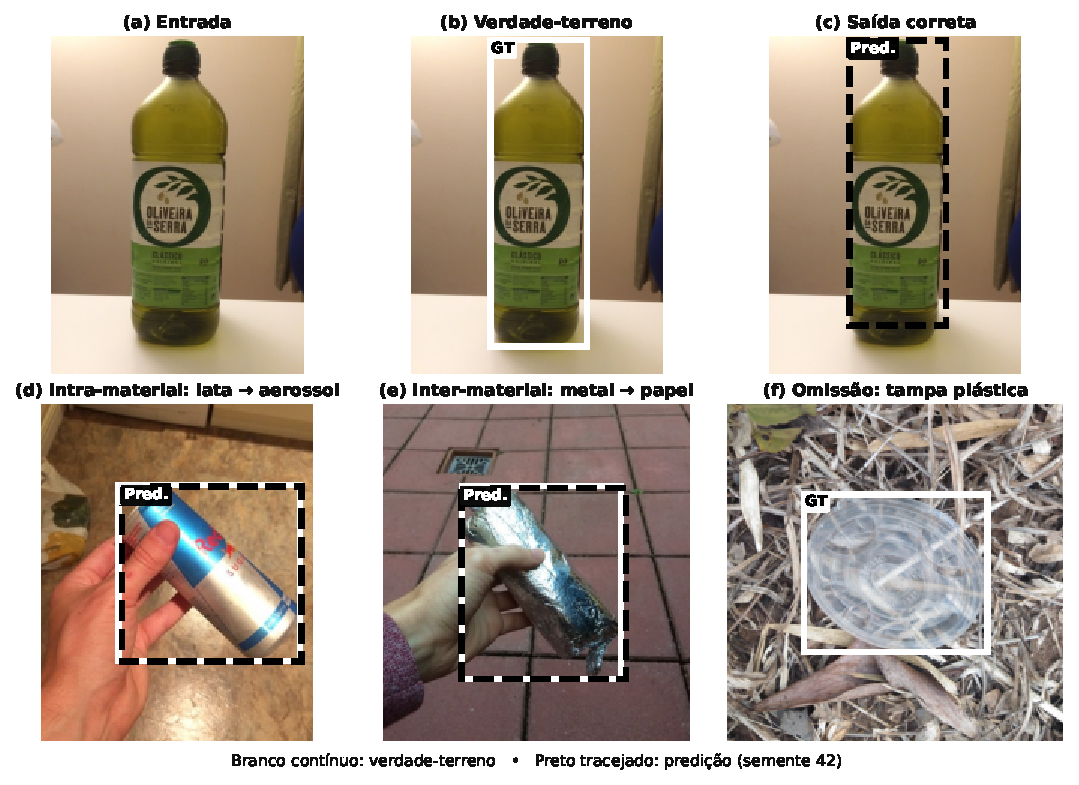
\includegraphics[width=\linewidth,trim=360 205 15 15,clip]{../paper/figures/qualitative_analysis.pdf}
      \vspace{0.08cm}\par
      {\fontsize{9.5}{11}\selectfont\textbf{GT = Pred.:} Other plastic bottle}
    \end{column}
    \begin{column}{0.235\textwidth}
      \centering{\color{ufpidark}\bfseries Intra-material}\par\vspace{0.10cm}
      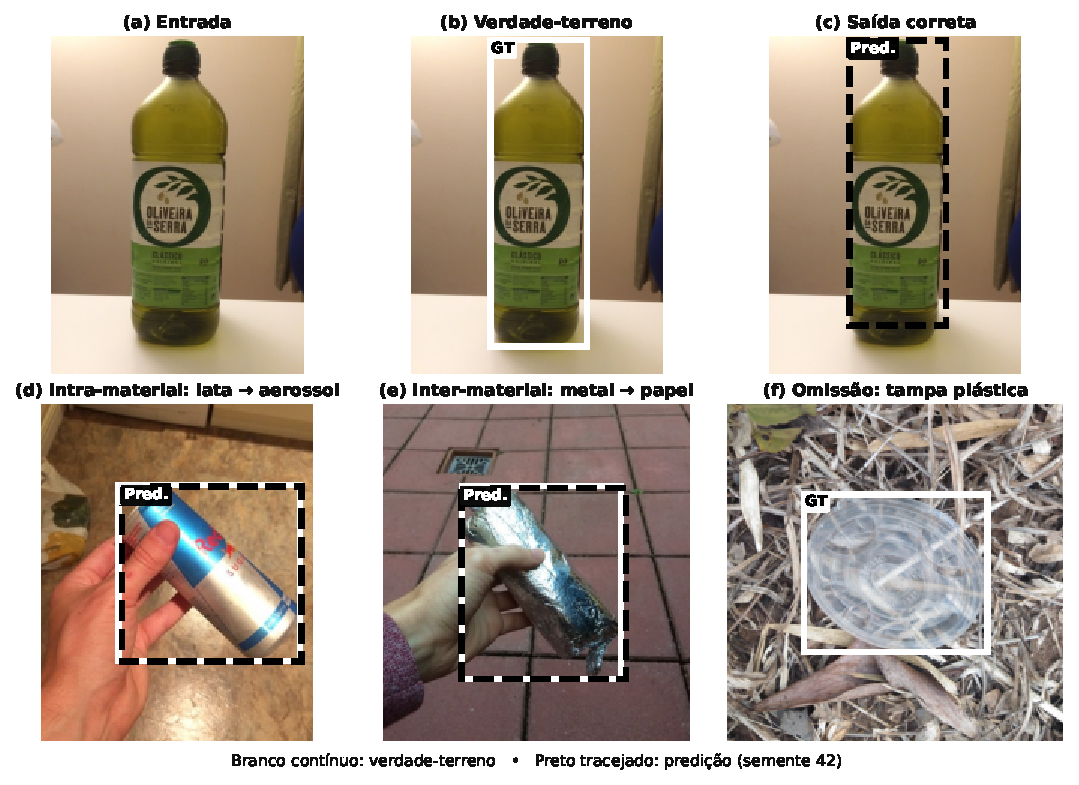
\includegraphics[width=\linewidth,trim=15 18 360 195,clip]{../paper/figures/qualitative_analysis.pdf}
      \vspace{0.08cm}\par
      {\fontsize{9.5}{11}\selectfont\textbf{GT:} Drink can\\\textbf{Pred.:} Aerosol}
    \end{column}
    \begin{column}{0.235\textwidth}
      \centering{\color{ufpidark}\bfseries Inter-material}\par\vspace{0.10cm}
      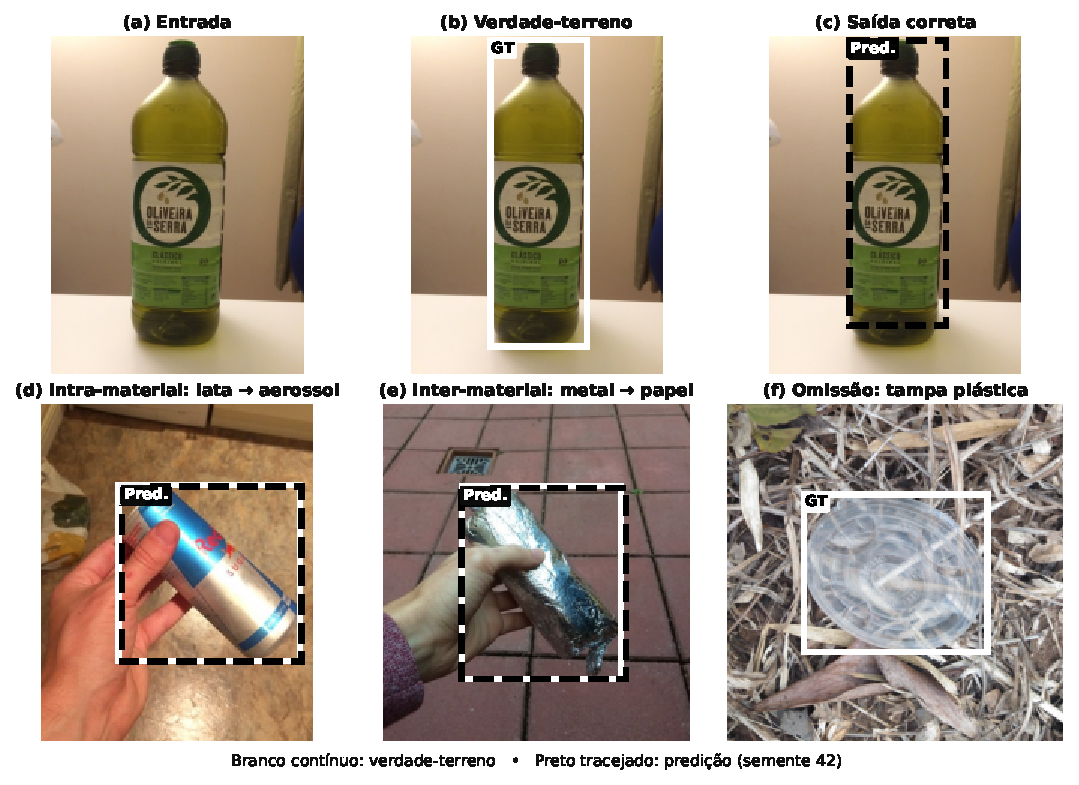
\includegraphics[width=\linewidth,trim=180 18 185 195,clip]{../paper/figures/qualitative_analysis.pdf}
      \vspace{0.08cm}\par
      {\fontsize{9.5}{11}\selectfont\textbf{GT:} Aluminium foil\\\textbf{Pred.:} Other carton}
    \end{column}
    \begin{column}{0.235\textwidth}
      \centering{\color{ufpidark}\bfseries Omissão}\par\vspace{0.10cm}
      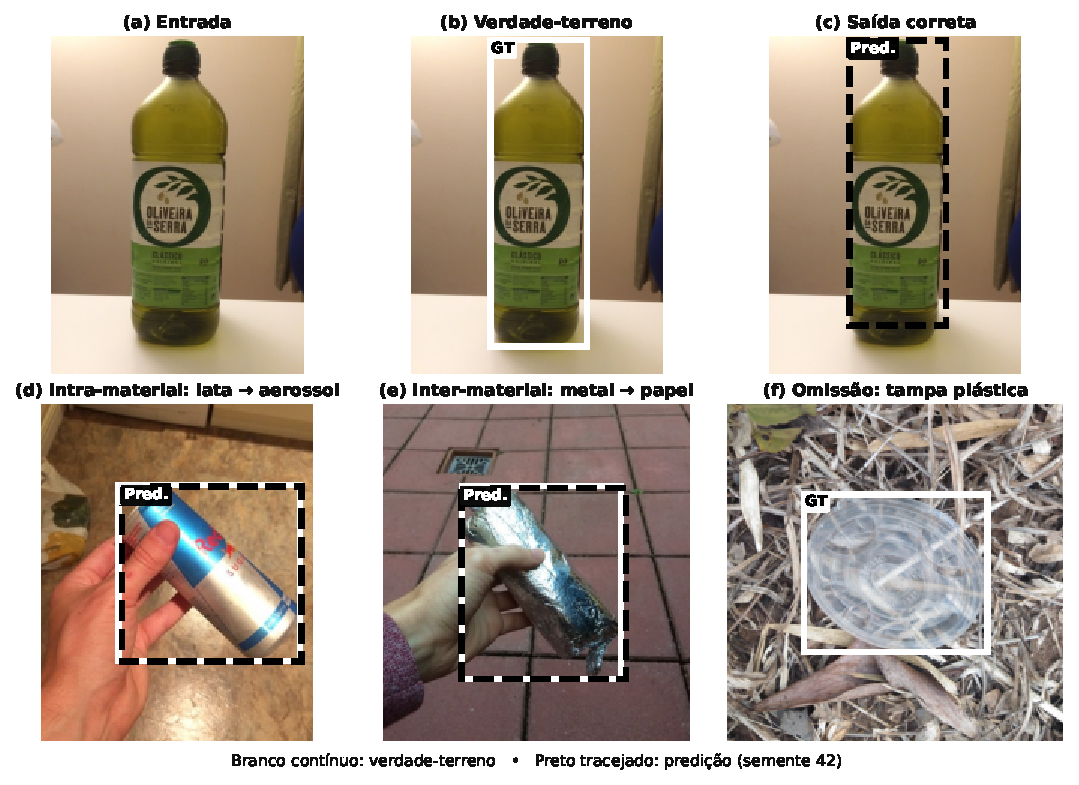
\includegraphics[width=\linewidth,trim=345 18 5 195,clip]{../paper/figures/qualitative_analysis.pdf}
      \vspace{0.08cm}\par
      {\fontsize{9.5}{11}\selectfont\textbf{GT:} Plastic lid\\\textbf{Pred.:} nenhuma}
    \end{column}
  \end{columns}
  \vspace{0.20cm}
  \centering{\color{muted}\fontsize{10}{12}\selectfont GT em branco; predição em preto tracejado. Semente 42.}
\end{frame}

% 12
\begin{frame}{Conclusões e limites}
  \begin{columns}[T,onlytextwidth]
    \begin{column}{0.58\textwidth}
      {\color{ufpidark}\fontsize{16.5}{19}\selectfont\bfseries Granularidade tem custo mensurável}\par
      \vspace{0.12cm}
      {\fontsize{12.5}{15}\selectfont Fine exige distinções difíceis em um conjunto pequeno e desbalanceado.}\par
      \vspace{0.24cm}

      {\color{ufpidark}\fontsize{16.5}{19}\selectfont\bfseries Material oferece um compromisso}\par
      \vspace{0.12cm}
      {\fontsize{12.5}{15}\selectfont Preserva informação de composição e melhora o ponto operacional.}\par
      \vspace{0.24cm}

      {\color{ufpidark}\fontsize{16.5}{19}\selectfont\bfseries Binary maximiza a detectabilidade}\par
      \vspace{0.12cm}
      {\fontsize{12}{14}\selectfont Sem distinção entre materiais.}
    \end{column}
    \begin{column}{0.36\textwidth}
      {\fontsize{16}{19}\selectfont\bfseries Limites do estudo}\par
      \vspace{0.15cm}
      \begin{itemize}
        \small
        \item uma partição fixa
        \item conjunto de teste com 225 imagens
        \item agrupamento por material definido no projeto
      \end{itemize}
      \vspace{0.22cm}
      {\color{muted}\fontsize{11.5}{14}\selectfont A taxonomia deve acompanhar a informação exigida pela aplicação.}
    \end{column}
  \end{columns}
\end{frame}

\end{document}
